\documentclass[lang=cn,11pt]{elegantpaper}
\usepackage{url}
\usepackage{booktabs}
\usepackage{multirow}
\usepackage{geometry}
\usepackage{longtable}
\usepackage{pdfpages}
\title{MDYSB5}
\date{}


\begin{document}

% 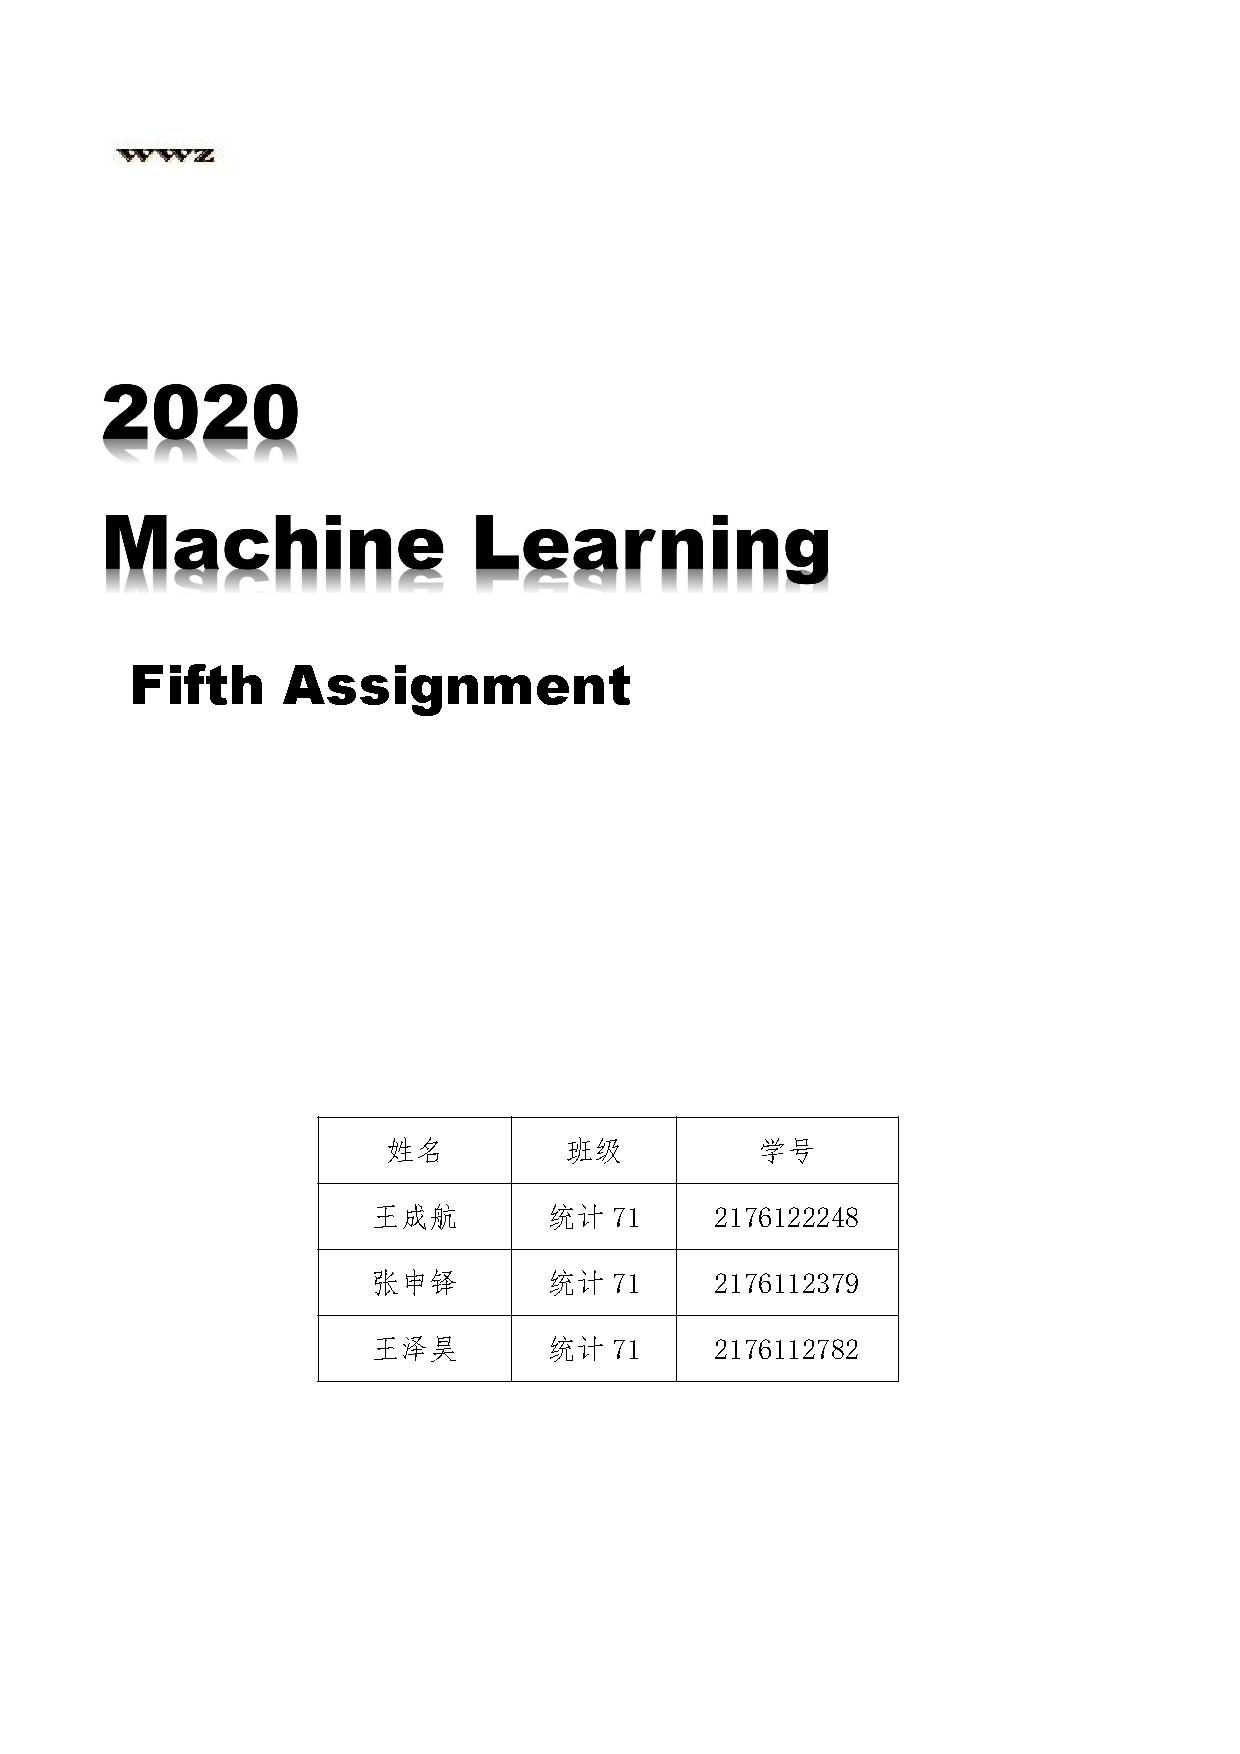
\includepdf[width=\paperwidth]{FM.pdf}
\newpage
\maketitle

	
\tableofcontents
\thispagestyle{empty}
\newpage
\normalsize
\pagenumbering{arabic}

\section{K-means用于图片压缩}
在日常生活中, 由于图像和视频本身的数据量非常大, 这就给给存储和传输带来了很多不便, 所以图像压缩和视频压缩得到了非常广泛的应用. 比如数码相机、USB 摄像头、可视电话视频点播、视频会议系统、数字监控系统等等, 都使用到了图像或视频的压缩技术. 在此, 下文将介绍一种使用k-means算法进行图像压缩的算法. 
\subsection{颜色量化算法(Color quantization algorithm)}
实际上, k-means进行图像压缩是一种颜色量化算法的实际应用. 颜色量化是利用人眼对颜色的惰性, 将原图像中不太重要的相似颜色合并为一种颜色, 减少图像中的颜色, 而使量化前后的图像对于人眼的认识误差最小, 即量化误差最小. 在彩色图像中, 每个像素的大小为3字节(RGB), 其中每种颜色的强度值都可以在0到255之间. 按照组合运算, 可以表示的颜色总数为256 $\times$ 256 $\times$ 256. 因此, 图像压缩的主要目标是使用颜色量化来压缩图像, 并且在图像的失真不是太明显的情况下减小图像的储存空间. 
\subsection{k-means压缩算法具体步骤}
\begin{figure}[ht]
    \centering
    \includegraphics[width=.8\textwidth]{Flow}
    \caption{算法流程图. \label{fig:flow}}
\end{figure}
首先, 考虑一个大小为128$\times$128$\times$3的图像. 如果对图片进行矢量化处理, 将得到一个大小为16384$\times$3的数组, 每一个元素代表原图像的R,G,B三个值组成的一个三维向量. 从而可以将图像视为许多个三维向量的数据集. 此时, 将K-Means应用于此数据集, 通过选择聚类中心的簇数$n$, 将$n$个最重要的质心选取出来. 用这个点的颜色取值来代替属于这一簇的元素的颜色. 这样, 只需保留少数质心的颜色数值, 剩下的点储存其属于哪一个质心便可. 从而对储存空间进行压缩. 

对于128$\times$128$\times$3的图像, 如果取k-means中的聚类簇数$k=16=2^4$, 即只使用16种颜色来对原图像进行颜色量化. 则新图像的总大小为$128\times128\times4 = 65536$, 这样, 储存空间在直观上得到了压缩. 

但由于需要储存16个质心的颜色值, 每个质心需要24位来储存, 因此, 总的储存空间为$65536 + 24 \times 16 = 65920$. 与原始图像进行比较, 原始图像所需的储存空间为$128 \times 128 \times 24 = 393216$位. 显然, 基于这样的方法, 理论上在$k=16$时可以将图片压缩至原图片大小的$16.76\%$. 

更一般的, 若原图像尺寸为$m\times n$, 选取聚类簇数为$k$, 则可将一般的RGB图像压缩为原图像的$$\frac{m\times n \times \log_2k+24\times k}{24\times m\times n}\times 100\%.$$
\subsection{实际表现}
基于以上的想法, 我们对于两张动物图片进行了压缩, 聚类簇数分别选为$k=8,\,16,\,32,\,64,\,128$. 首先, 对于第一张图片进行了压缩, 得到的结果分别如 \figref{fig:cat1}.

\begin{figure}[ht]
    \centering
    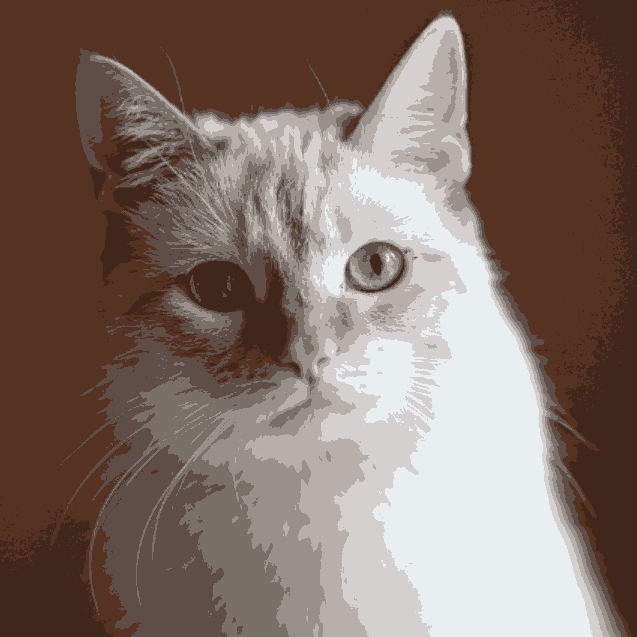
\includegraphics[width=.3\textwidth]{cat1/8.png}
    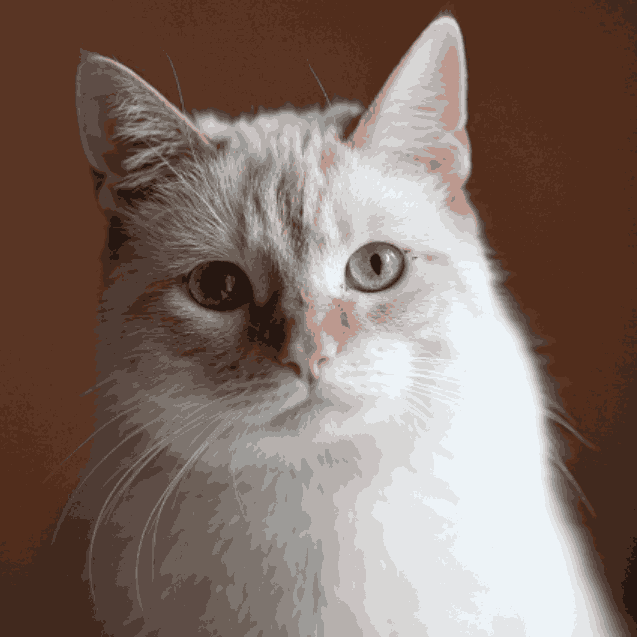
\includegraphics[width=.3\textwidth]{cat1/16.png}
    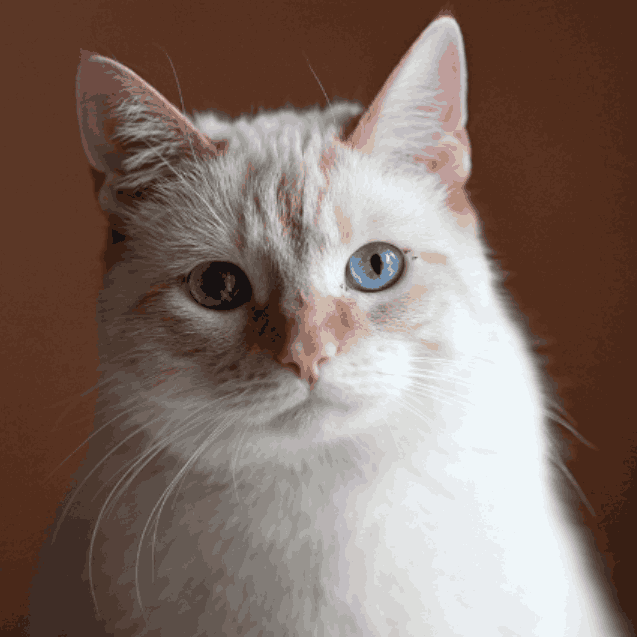
\includegraphics[width=.3\textwidth]{cat1/32.png}\\

    \vspace{2pt}
    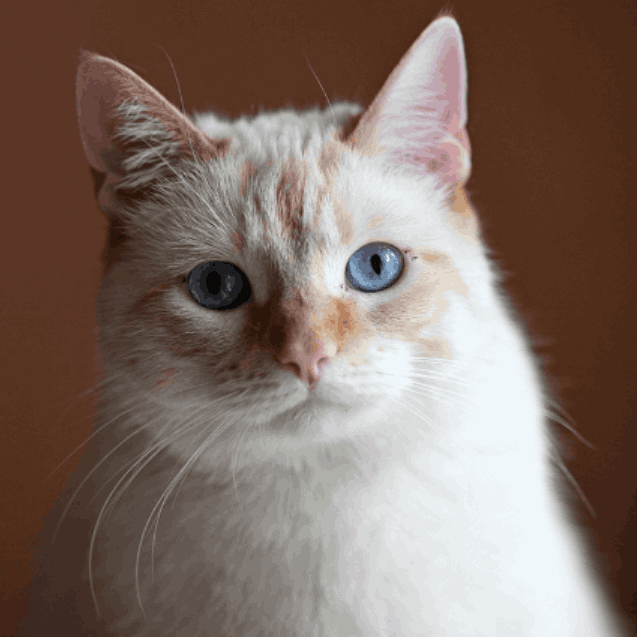
\includegraphics[width=.3\textwidth]{cat1/64.png}
    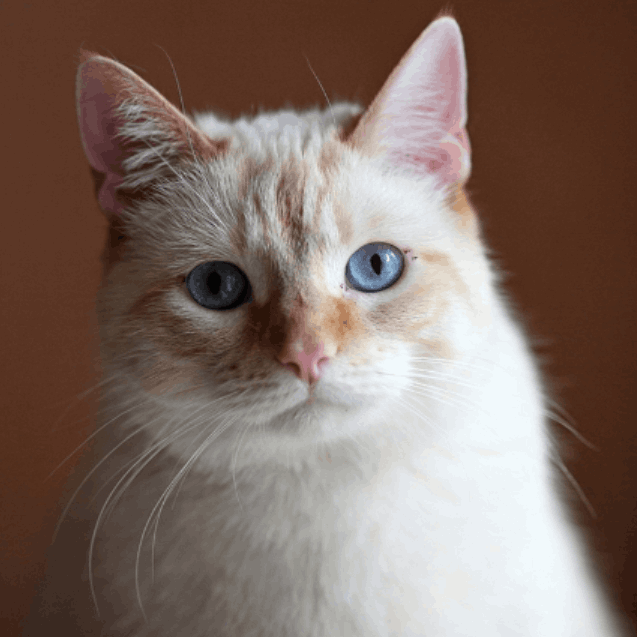
\includegraphics[width=.3\textwidth]{cat1/128.png}
    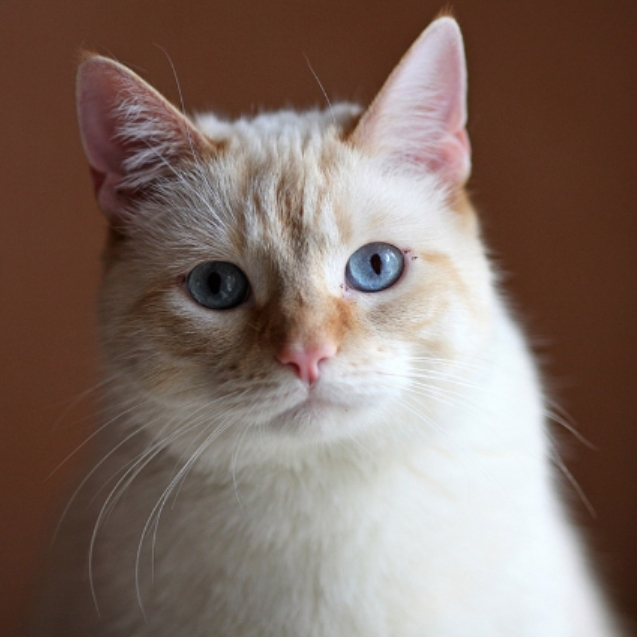
\includegraphics[width=.3\textwidth]{cat1/Origin.png}
    \caption{从左到右、从上到下$k$的值依次增加, 最后一张图为原图. \label{fig:cat1}}
\end{figure}

每张图片的大小如下表所示
\begin{table}[h]
    \centering
    \begin{tabular}{c|ccccc}
    \hline
    图片大小 (字节)  & $k=8$   & $k=16$   & $k=32$   & $k=64$   & $k=128$  \\ \hline
    682078   & 45197 & 75804  & 123399 & 165238 & 237626 \\
    压缩比 (\%) & 6.626 & 11.114 & 18.092 & 24.226 & 34.839 \\ \hline
    \end{tabular}
\end{table}

\begin{figure}[ht]
\centering
  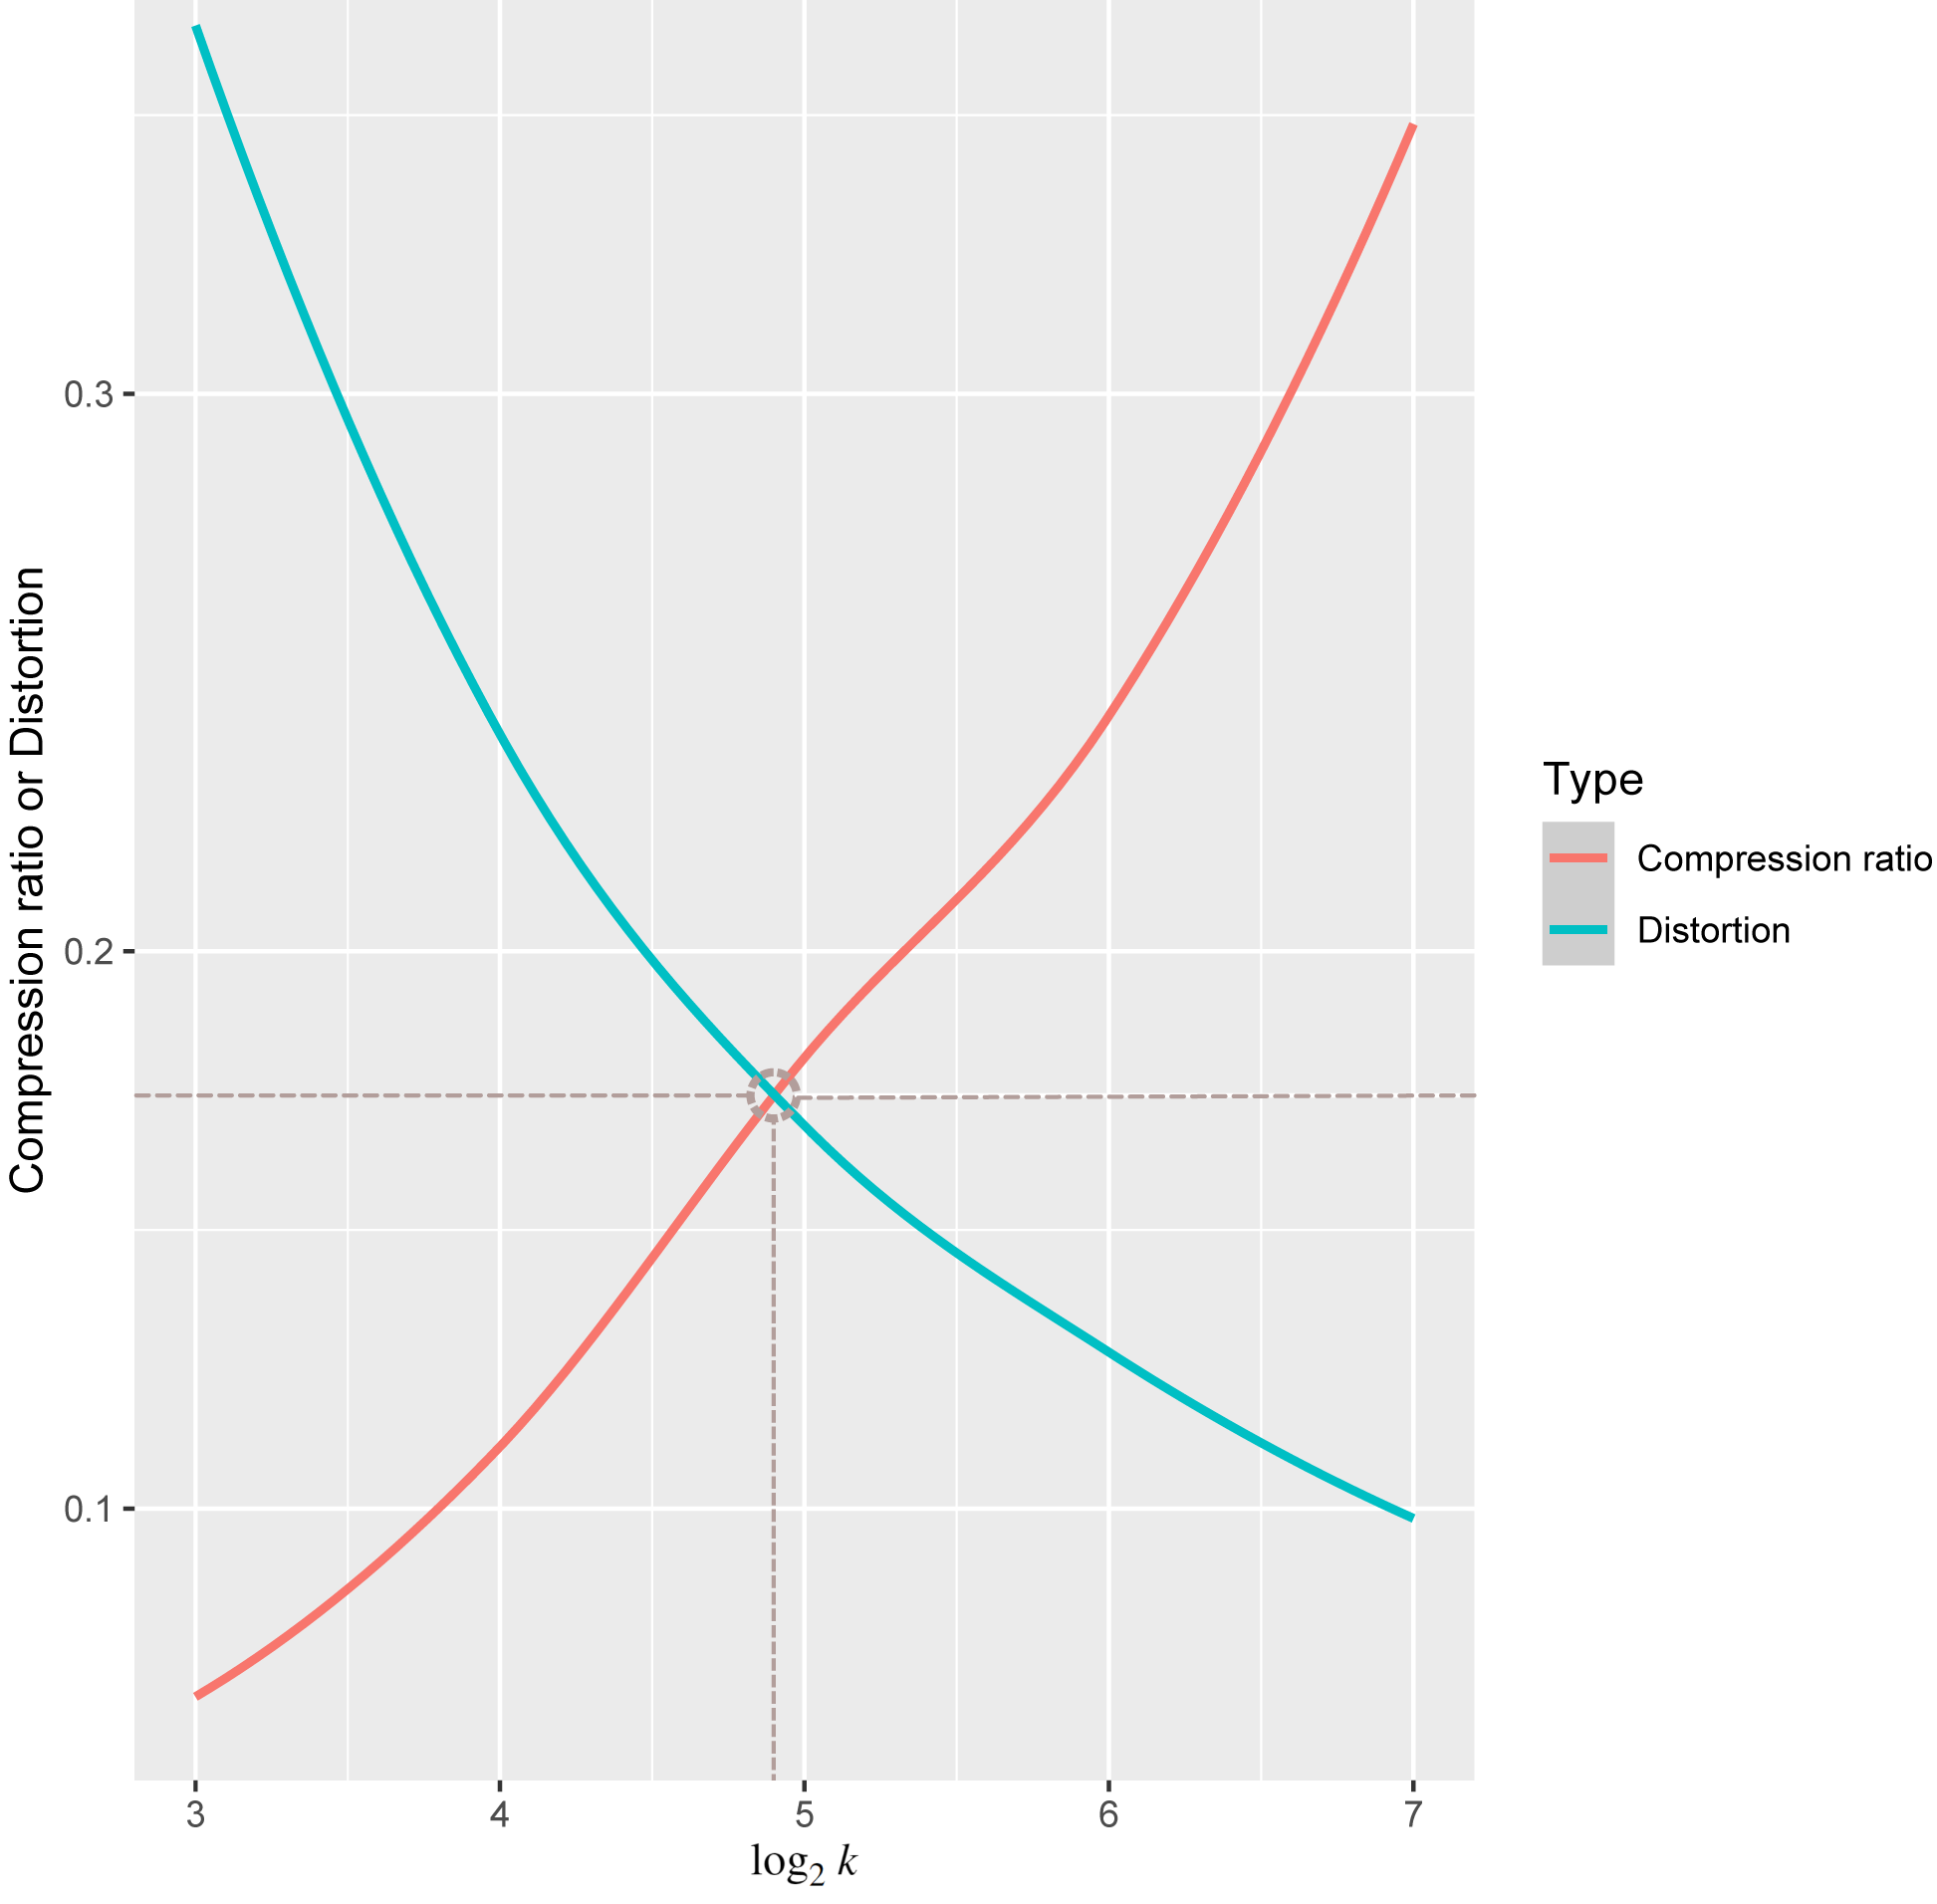
\includegraphics[width=0.9\textwidth]{cat1to}
  \caption{\label{cat2tradeoff}}
\end{figure}




从图中可以看出, 实际上$k$取64甚至32时, 压缩过的图片就已经大致和原图相似了. 第1至3张图片中因为颜色数较少, 未能表现出猫眼的真实颜色, 但对猫毛的颜色刻画逐渐生动, 到第4张时已经非常接近原图给人的视觉观感. 

之后, 对于第二张图片进行了压缩, 得到的结果分别如 \figref{fig:cat2}.

\begin{figure}[ht]
    \centering
    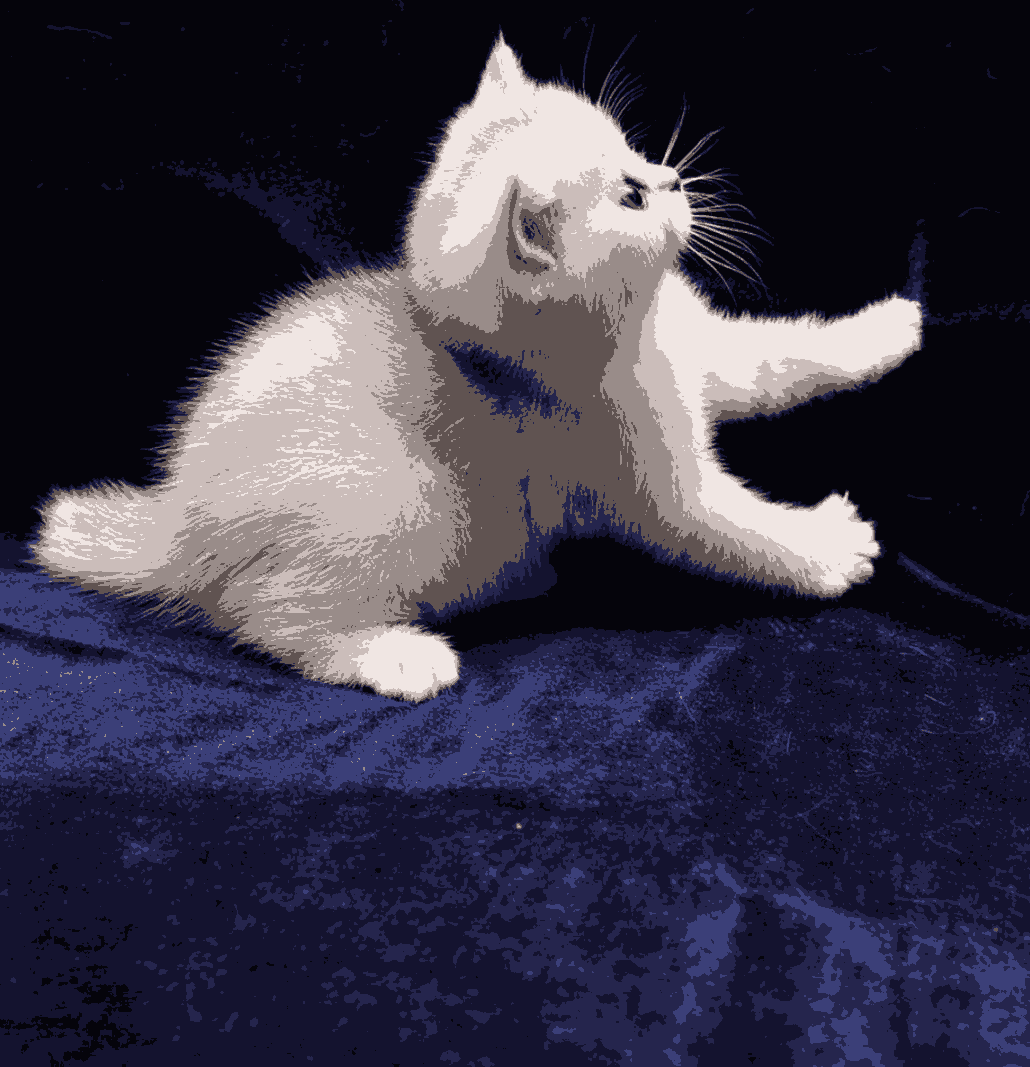
\includegraphics[width=.3\textwidth]{cat2/8.png}
    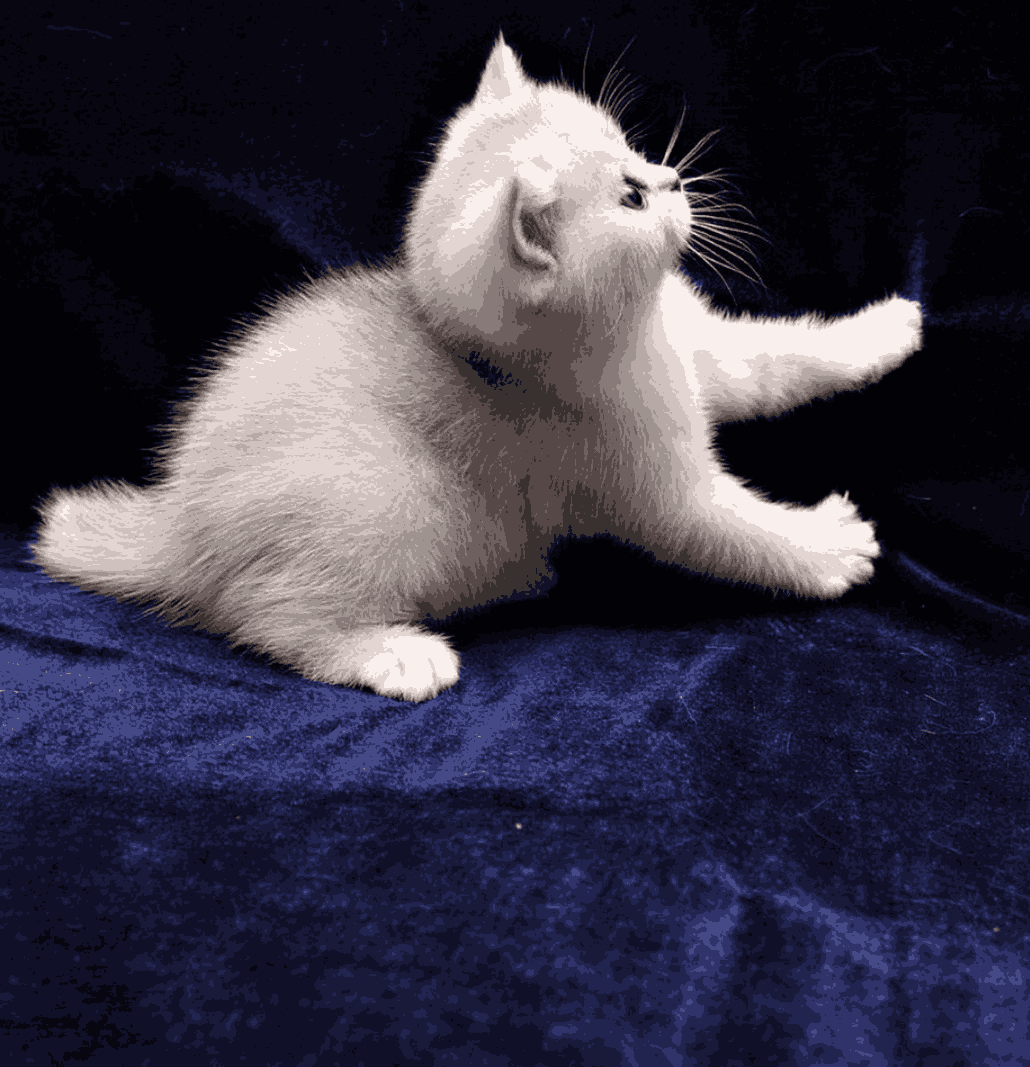
\includegraphics[width=.3\textwidth]{cat2/16.png}
    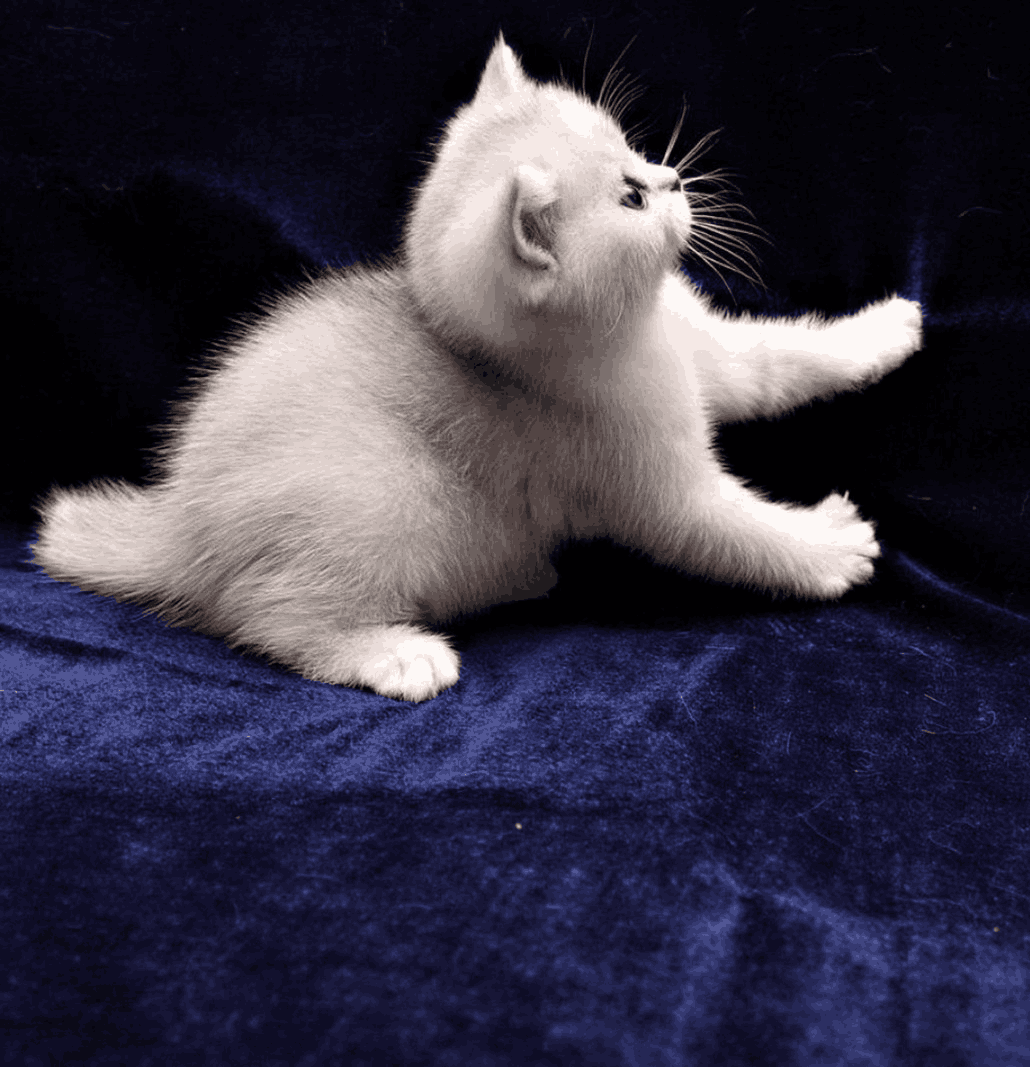
\includegraphics[width=.3\textwidth]{cat2/32.png}\\

    \vspace{2pt}
    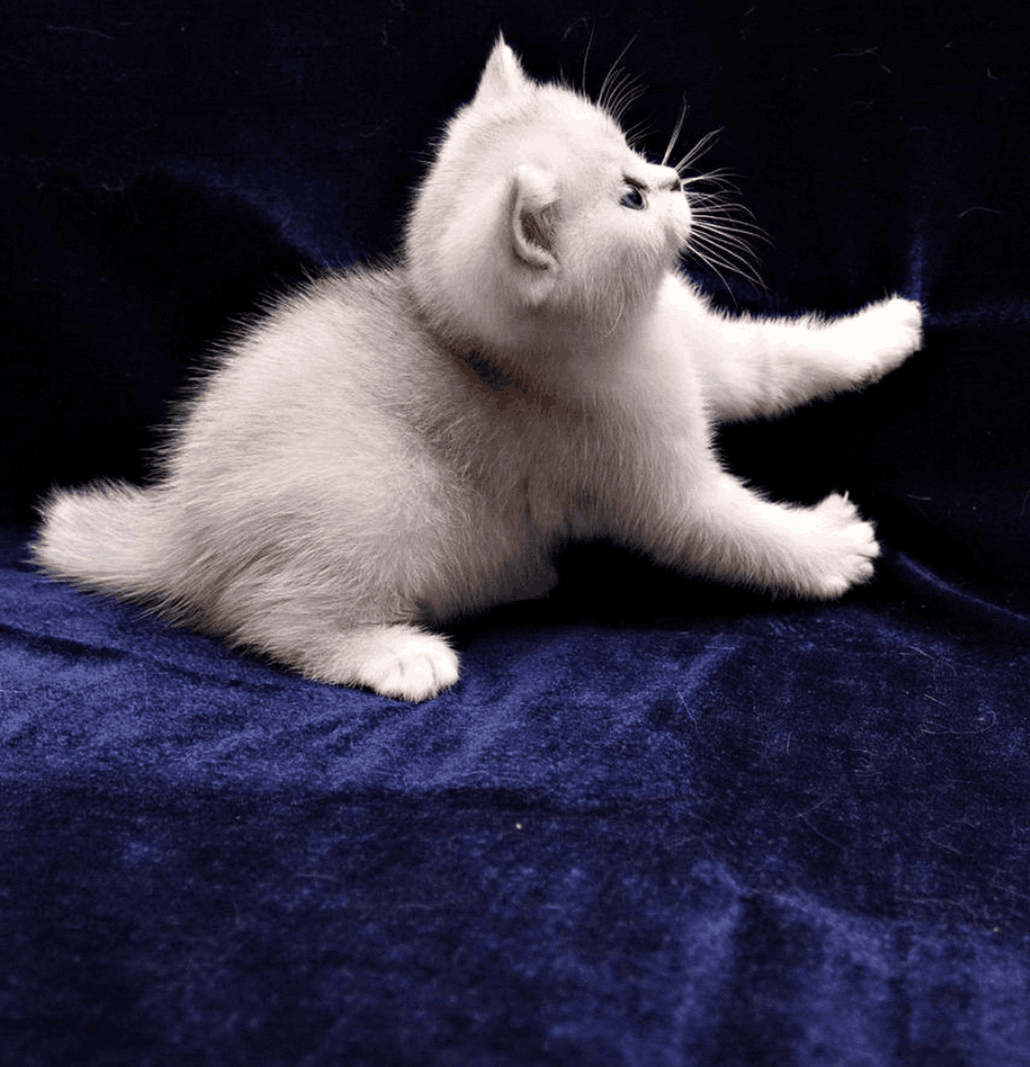
\includegraphics[width=.3\textwidth]{cat2/64.png}
    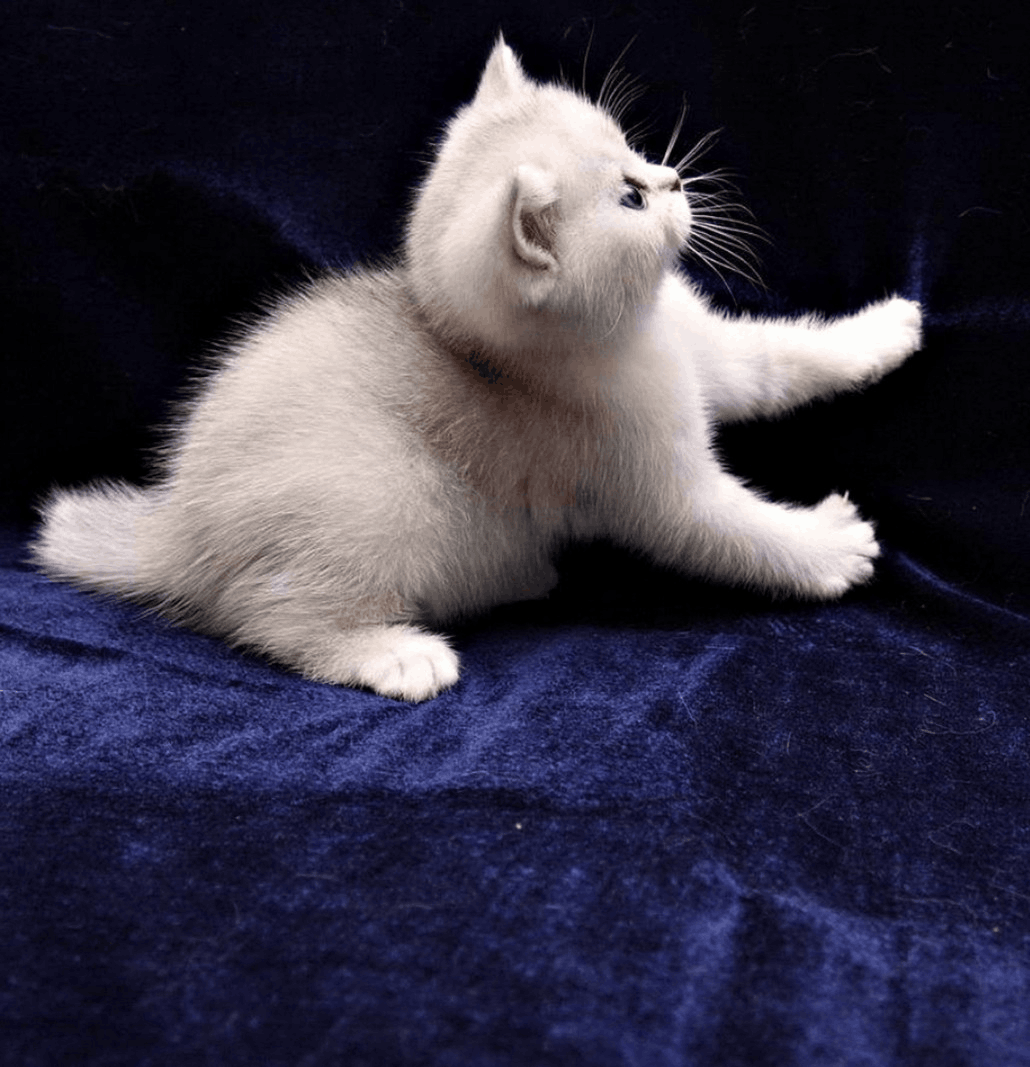
\includegraphics[width=.3\textwidth]{cat2/128.png}
    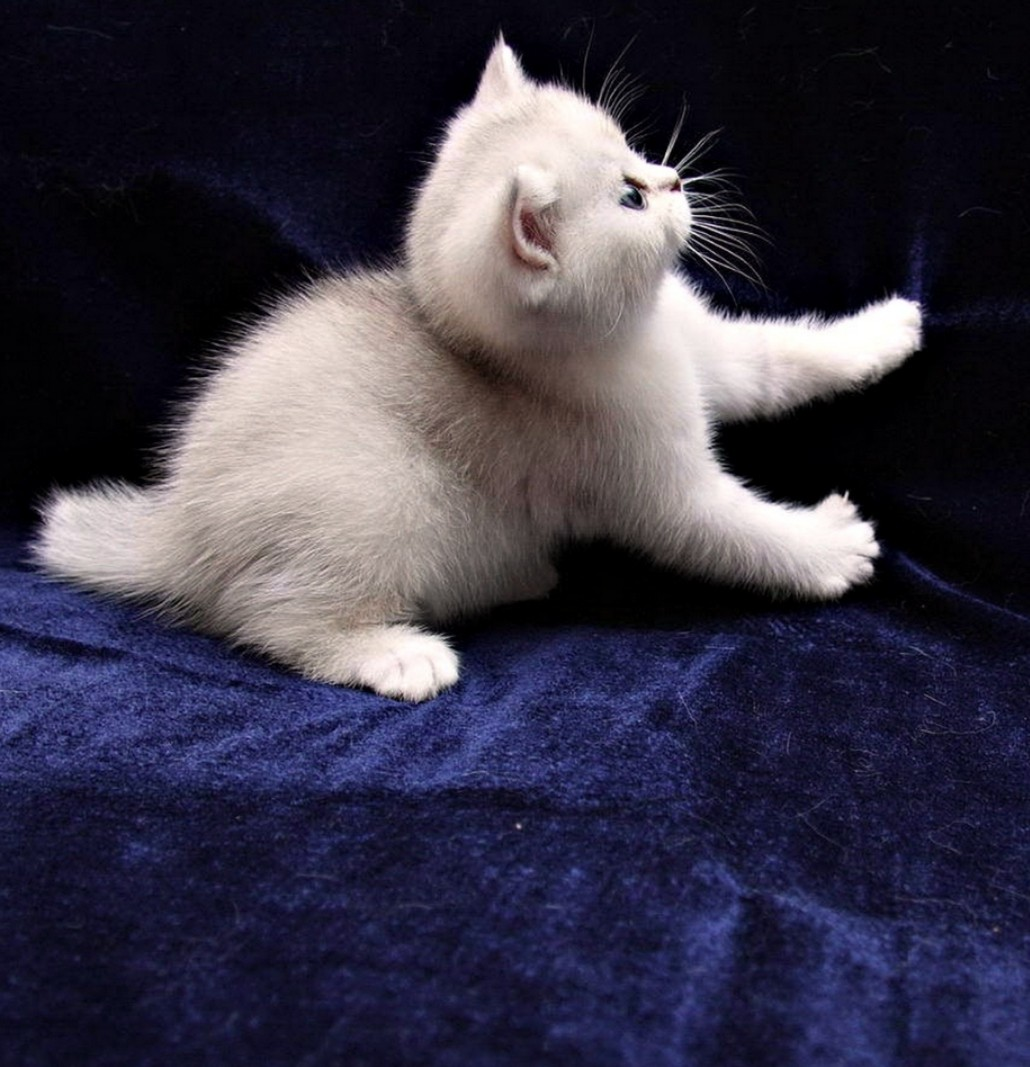
\includegraphics[width=.3\textwidth]{cat2/Origin.png}
    \caption{从左到右、从上到下$k$的值依次增加, 最后一张图为原图. \label{fig:cat2}}
\end{figure}

每张图片的大小如下表所示
\begin{table}[ht]
    \centering
    \begin{tabular}{c|ccccc}
    \hline
    图片大小 (字节)  & $k=8$    & $k=16$   & $k=32$   & $k=64$   & $k=128$  \\ \hline
    1140062  & 132802 & 248046 & 428423 & 656589 & 874825 \\
    压缩比 (\%) & 11.647 & 21.757 & 37.579 & 57.592 & 76.735 \\ \hline
    \end{tabular}
\end{table}

相比于 \figref{fig:cat1}, \figref{fig:cat2} 的颜色构成较为简单, 主色即为蓝、白、黑, 所以可以看出在第2张图中, 只使用8种颜色时, 便已经可以基本表现出猫毛、猫眼等主要特征, 虽然在色彩交界处出现了比较明显的断层. 不过它的大小仅为原图的1/10, 可以说是一种比较高效的图像压缩方式. 



\begin{figure}[ht]
\centering
  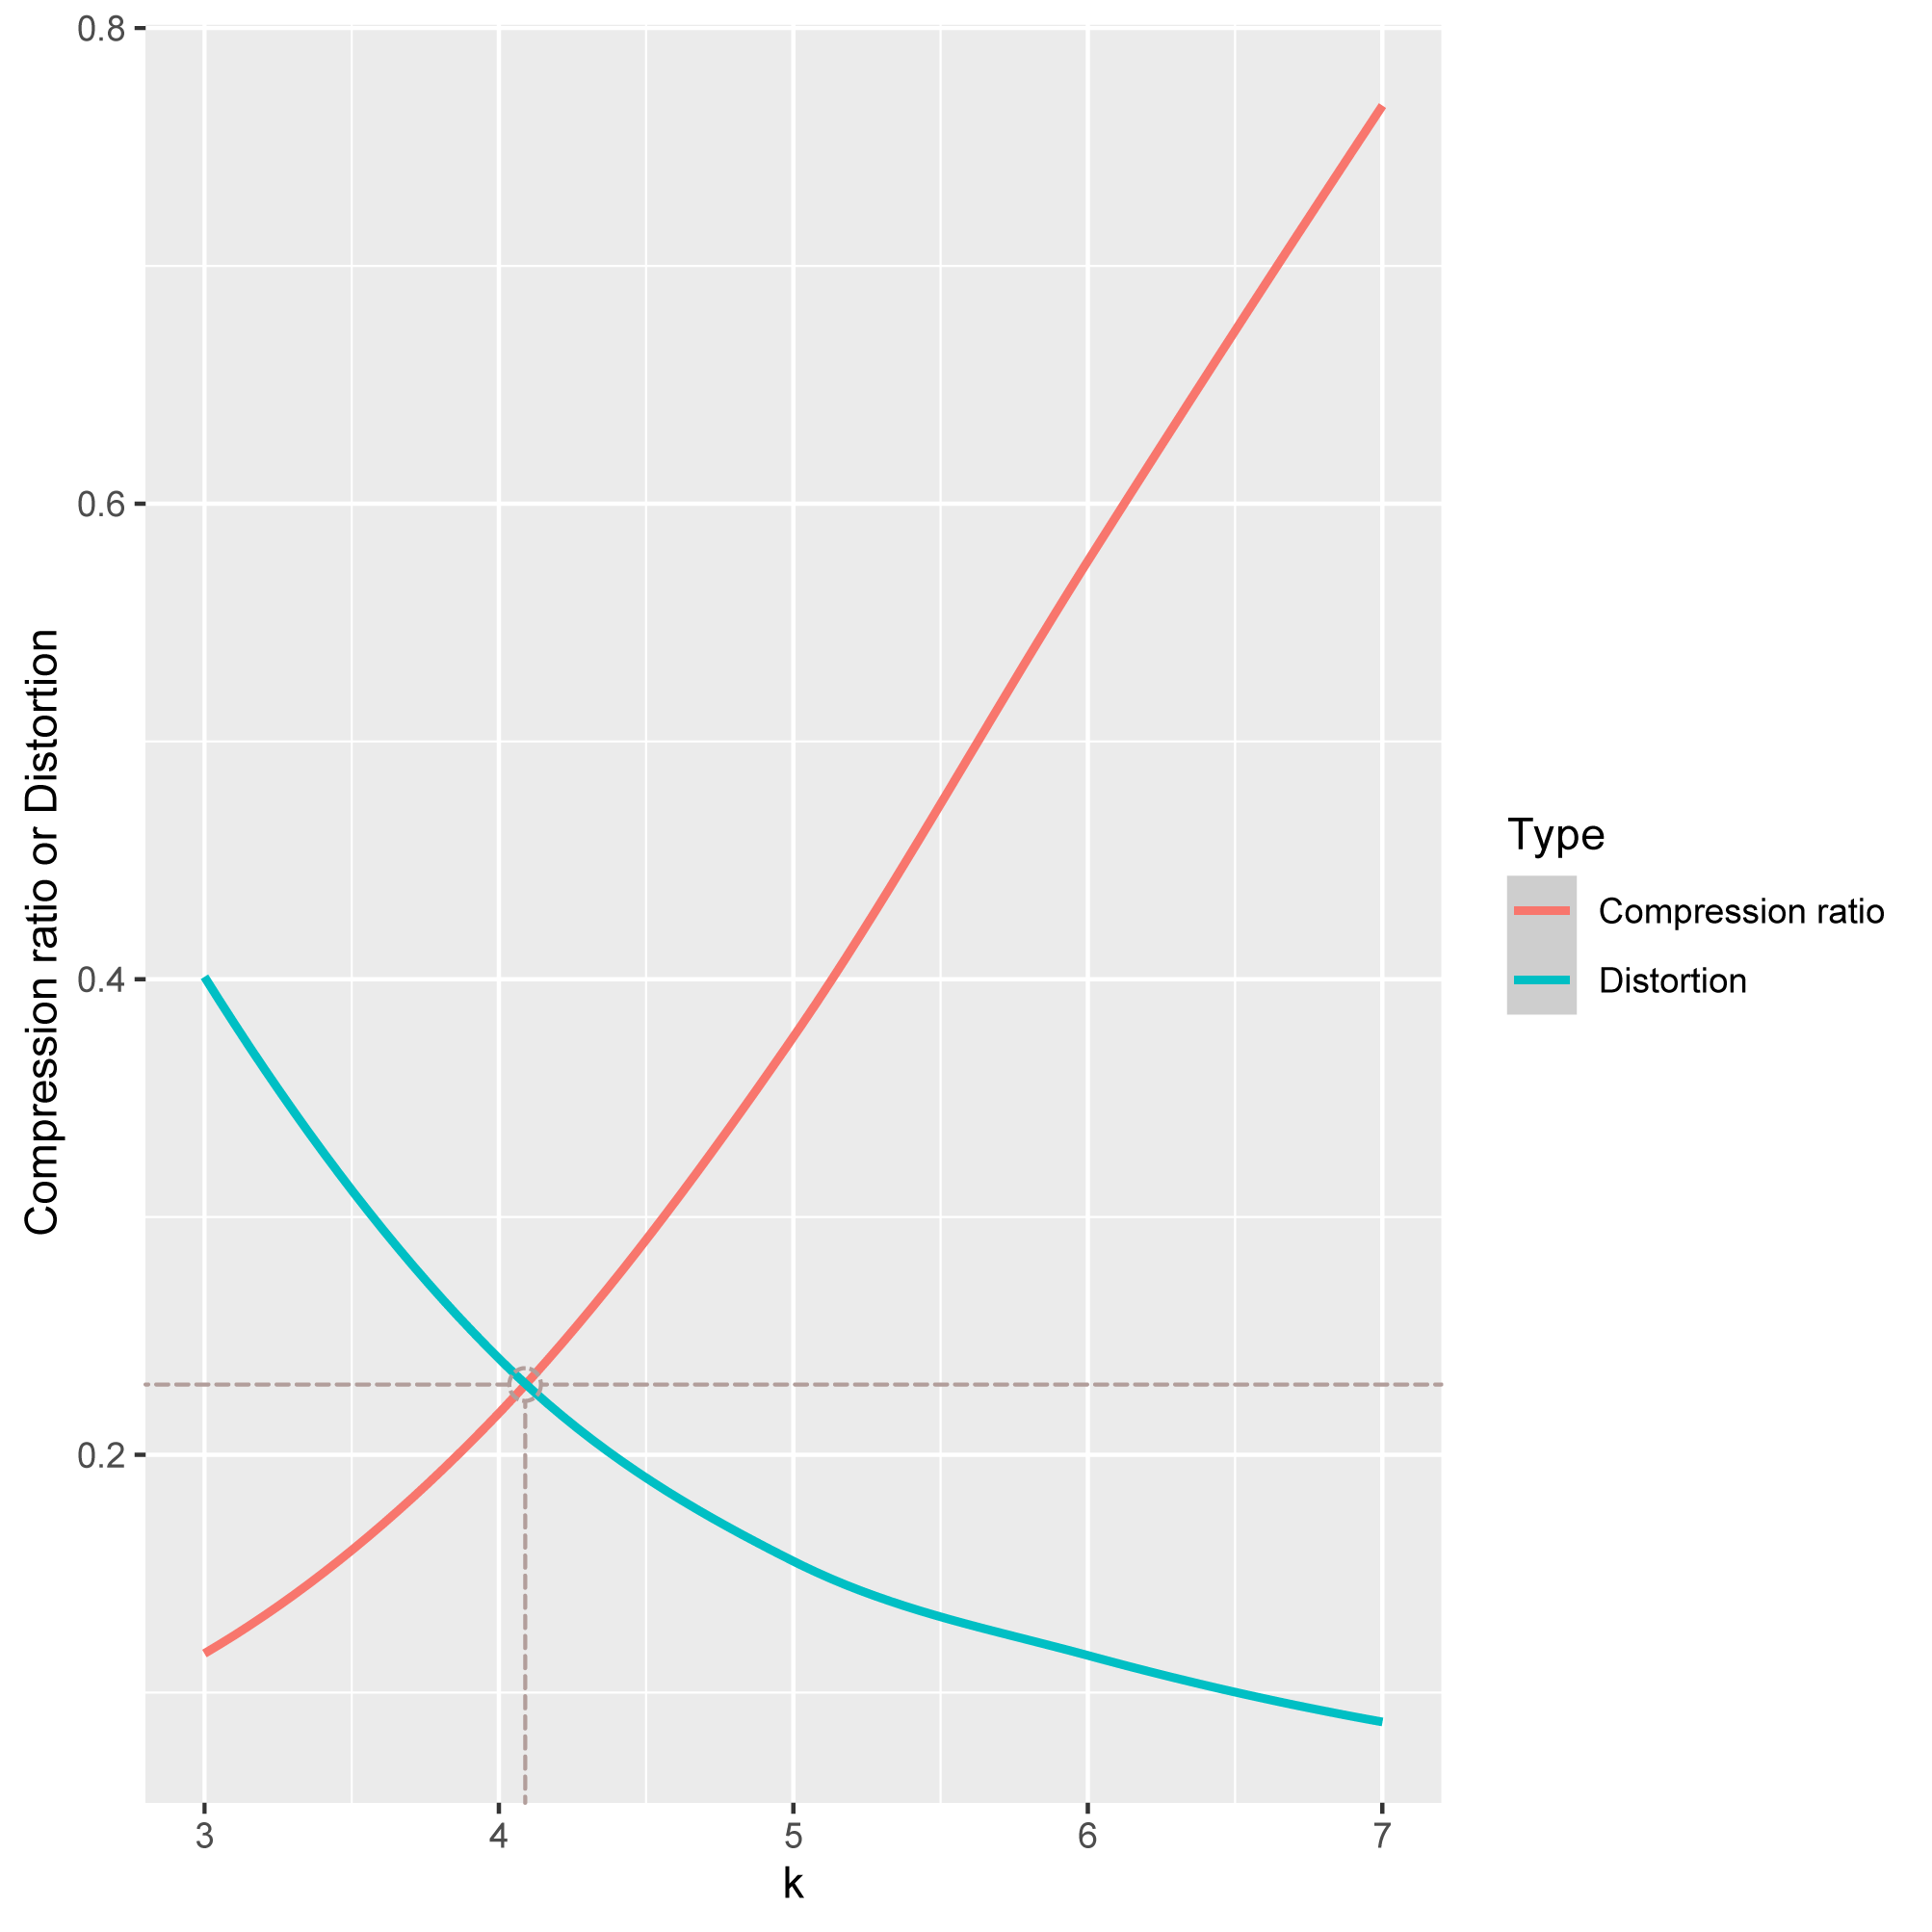
\includegraphics[width=0.9\textwidth]{cat2to}
  \caption{\label{cat2tradeoff}}
\end{figure}







但k-means图像压缩仍是一种有损的图像压缩方式, 即以牺牲一些图像信息为代价减少图片大小, 目前也已经有了各种无损的压缩图片技术, 但多半都有压缩比率不高的问题存在, 但我们相信随着科学技术的发展, 会有更加完善的无损压缩技术出现. 










\section{FCM和KFCM算法在图像分割中的应用及对比}
\Huge 这几个引用明天查一下

\normalsize
K-means算法可以看作高斯混合聚类在混合成分方差相等、且每个样本仅指派给一个混合成分时的特例. 而基于K-means的思想也继而衍生了很多变体, 如k-medoids算法[Kaufman and Rousseeuw,1987]强制原型向量必为训练样本, k-mosed算法[Huang,1988]可处理离散属性. FCM[Bezdek,1981]则是“软聚类”算法, 允许每个样本以不同程度属于多个原型. 引入核技巧则可得KFCM算法. 
\subsection{FCM算法}
\begin{equation*}
J(\theta)=\sum_{i=1}^k\sum_{k=1}^N d^2(x_k,\theta_i)
\end{equation*}
\\ 模糊聚类算法对象函数的数学模型为:
\begin{equation*}
	J(U,\theta)=\sum_{i=1}^c\sum_{k=1}^Nu_{ik}^m d^2(x_k,\theta_i)
\end{equation*}
其中$m$为模糊指数,$m>1$,$U$为隶属度矩阵,$\mu_{ik}$为隶属度(即$U$的元素),
\ $d(\ \cdot \ , \ \cdot \ )$为不相似测度函数,$x_k$是输入样本特征,$\theta_i$是聚类中心,$N$是输入样本(即图像像素)总数,$c$为聚类数目。
\par 聚类的过程是通过调整$U$和$\theta$使上式的求和值最小化。可以理解这个最小化过程是一个聚类过程:要使该求和式最小,则要求其中的每一乘积项最小,就是说,$d(\ \cdot \ , \ \cdot \ )$大的项,要由小的$\mu_{ik}$与其相乘。换言之,样本与聚类中心越不相似,则要求该样本对这个聚类中心的隶属度越小,反之,则隶属度越大。由此看出上式的收敛过程就是一个聚类过程。
\par 对比K-means与FCM的目标函数,可以知道,K-means是排他性聚类算法,即一个数据点只能属于一个类别,而FCM只计算数据点雨各个类别的相似度,即对于任意一个数据点,使用K-means算法,其属于某个类别非否即是,而对于FCM算法,其属于某个类别的相似度只是一个百分比。





\newpage
\nocite{*}

\bibliographystyle{unsrt}
\bibliography{wpref}

\end{document}
